\documentclass[a4paper]{article}

%% Language and font encodings
\usepackage[english]{babel}
\usepackage[utf8x]{inputenc}
\usepackage[T1]{fontenc}

%% Sets page size and margins
\usepackage[a4paper,top=3cm,bottom=2cm,left=3cm,right=3cm,marginparwidth=1.75cm]{geometry}

%% Useful packages
\usepackage{amsmath}
\usepackage{graphicx}
\usepackage[colorinlistoftodos]{todonotes}
\usepackage[colorlinks=true, allcolors=blue]{hyperref}

\title{Your Paper}
\author{You}

\begin{document}
\maketitle

\begin{abstract}
Your abstract.
\end{abstract}

\section{Introduction}

Your introduction goes here! 

\section{Some examples to get started}

\subsection{How to add Comments}

Everything on a line after a \% sign is a comment:

%
% Here's an example comment!
%

\subsection{How to include Figures}

First you have to upload the image file from your computer using the upload link the project menu in Overleaf. Then use the "includegraphics" command to include it in your document. Use the figure environment and the caption command to add a number and a caption to your figure. Use the "ref" command to cite the figure number in the text of your article. See the code for Figure \ref{fig:frog} in this section for an example.

\begin{figure}
\centering
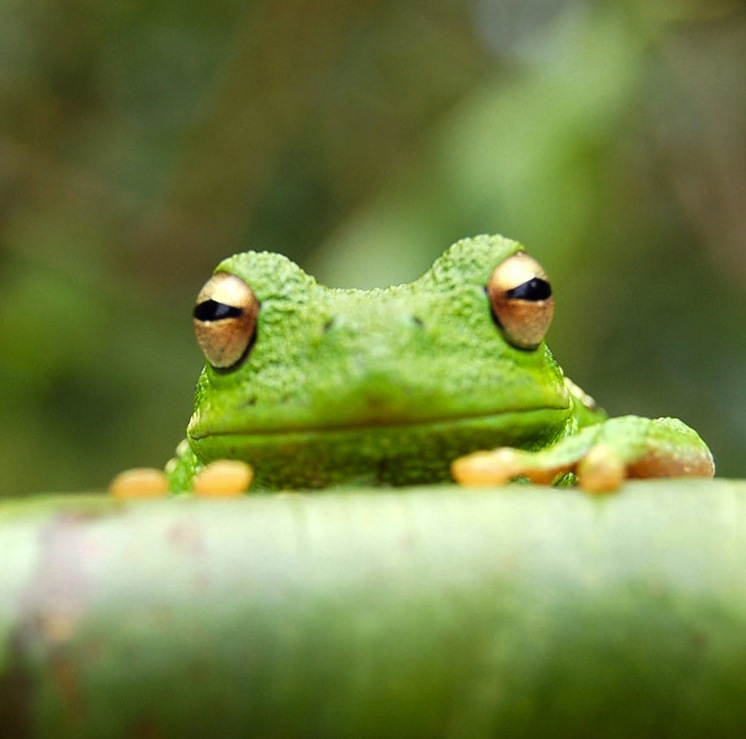
\includegraphics[width=0.3\textwidth]{frog.jpg}
\caption{\label{fig:frog}This frog was uploaded via the project menu.}
\end{figure}

\subsection{How to add Tables}

Use the table and tabular commands for basic tables --- see Table~\ref{tab:widgets}, for example. 

\begin{table}
\centering
\begin{tabular}{l|r}
Item & Quantity \\\hline
Widgets & 42 \\
Gadgets & 13
\end{tabular}
\caption{\label{tab:widgets}An example table.}
\end{table}

\subsection{How to write Mathematics}

\LaTeX{} is great at typesetting mathematics. Let $X_1, X_2, \ldots, X_n$ be a sequence of independent and identically distributed random variables with $\text{E}[X_i] = \mu$ and $\text{Var}[X_i] = \sigma^2 < \infty$, and let
\[S_n = \frac{X_1 + X_2 + \cdots + X_n}{n}
      = \frac{1}{n}\sum_{i}^{n} X_i\]
denote their mean. Then as $n$ approaches infinity, the random variables $\sqrt{n}(S_n - \mu)$ converge in distribution to a normal $\mathcal{N}(0, \sigma^2)$.

Similarly, you can right multiline equations using the "align" environment:
\begin{align*}
5 \cdot (3 + 2) & = 5 \cdot 3 + 5 \cdot 2 \\
& = 15 + 10 \\
& = 25
\end{align*}



\subsection{How to add Citations and a References List}

To add a reference, put the bibliography information into a "bibitem" in the bibliography section.  To cite it, use the "cite" Latex command.

Example: 

In 1947, Artin gave a presentation for the braid group in terms of generators and relations \cite{A}.

\begin{thebibliography}{9999}

%% \bibitem{AMU} J.\ E.\ Andersen, G.\ Masbaum, and K.\ Ueno, \emph{Topological Quantum Field Theory and the Nielsen-Thurston classification of M(0,4)}, Math.\ Proc.\ Cambridge Philos.\ Soc., \textbf{141} (2006), no. 3, 477--488.

\bibitem{A} E.\ Artin, \emph{The theory of braids}, Ann. of Math. (2) \textbf{48} (1947), %101-126.

\bibitem{BK} B.\ Bakalov and A.\ Kirillov, Jr., {\em Lectures on
Tensor Categories and Modular Functors}, University Lecture Series,
vol.\ {\bf 21},  Amer.\ Math.\ Soc., 2001.

\bibitem{hep-th/9311155} J.\ Barrett and B.\ Westbury. {\em Invariants
of Piecewise-Linear 3-Manifolds}, Trans.\ Amer.\ Math.\ Soc.\ \textbf{348} (1996), 3997--4022.
\end{thebibliography}


\end{document}
